% !TeX program = xelatex
\documentclass{article}
\usepackage{kotex}
\usepackage[a4paper,left=3cm, right=3cm, top=2cm, bottom=2cm]{geometry}
\usepackage{amsmath}
\usepackage{graphicx}
\usepackage{caption}
\usepackage{setspace}
\usepackage{xcolor}
\usepackage{titlesec}
\usepackage{amssymb}
\usepackage{tcolorbox}
\usepackage{amsthm}
\usepackage{multirow}
\usepackage{array}
\usepackage{tikz}
\usetikzlibrary{positioning,arrows.meta,calc}
\usepackage{pgfplots}
\pgfplotsset{compat=1.18}

\title{7.1 Orthogonal Matrices}
\date{}
\author{}
\setstretch{1.3}

\titleformat{name=\section, numberless}
  {\normalfont\large\bfseries\color{blue}}{}
  {0pt}{}
\geometry{a4paper, margin=1in}

\newcommand{\redheading}[1]{{\vspace{2mm}\noindent\Large\bfseries\color{red!55!black} #1\par}\vspace{2mm}}

\newtheoremstyle{mystyle}
  {}{}{\itshape}{}{\bfseries}{.}{.5em}{}
\theoremstyle{mystyle}

\begin{document}
\maketitle

\begin{tcolorbox}[colback=blue!5, colframe=blue!60!black,
  title=Chapter 7: Diagonalization and Quadratic Forms --- Overview,
  boxrule=0.5mm, arc=3mm]
Section 5.2 gave conditions for diagonalizability of $n\times n$ matrices without
identifying which classes actually satisfy them. This chapter shows that \emph{every
symmetric matrix is diagonalizable} --- an important result exploited across many
applications.
\end{tcolorbox}

{\itshape\color{blue!45!black}
In this section we discuss the class of matrices whose inverses can be obtained by
transposition. Such matrices occur in a variety of applications and arise as transition
matrices when one orthonormal basis is changed to another.\par}

\vspace{2mm}

\redheading{Orthogonal Matrices}

\begin{tcolorbox}[colback=teal!4, colframe=teal!65!black,
  title={\textbf{Definition 1}}, boxrule=0.5mm, arc=3mm]
A square matrix $A$ is \textbf{orthogonal} if its transpose equals its inverse:
\[
  A^{-1} = A^T, \quad\text{or equivalently,}\quad AA^T = A^TA = I \tag{1}
\]
A matrix transformation $T_A\colon\mathbb{R}^n\to\mathbb{R}^n$ is an
\textbf{orthogonal transformation} (or \textbf{orthogonal operator}) if $A$ is orthogonal.
\end{tcolorbox}

\subsection*{EXAMPLE 1 | A $3\times3$ Orthogonal Matrix}

The matrix
\[
  A = \begin{bmatrix}
        \tfrac{3}{7} & \tfrac{2}{7} & \tfrac{6}{7}\\[4pt]
        -\tfrac{6}{7} & \tfrac{3}{7} & \tfrac{2}{7}\\[4pt]
        \tfrac{2}{7} & \tfrac{6}{7} & -\tfrac{3}{7}
      \end{bmatrix}
\]
is orthogonal since
\[
  A^T A =
  \begin{bmatrix}
    \tfrac{3}{7} & -\tfrac{6}{7} & \tfrac{2}{7}\\[4pt]
    \tfrac{2}{7} & \tfrac{3}{7} & \tfrac{6}{7}\\[4pt]
    \tfrac{6}{7} & \tfrac{2}{7} & -\tfrac{3}{7}
  \end{bmatrix}
  \begin{bmatrix}
    \tfrac{3}{7} & \tfrac{2}{7} & \tfrac{6}{7}\\[4pt]
    -\tfrac{6}{7} & \tfrac{3}{7} & \tfrac{2}{7}\\[4pt]
    \tfrac{2}{7} & \tfrac{6}{7} & -\tfrac{3}{7}
  \end{bmatrix}
  = \begin{bmatrix}1&0&0\\0&1&0\\0&0&1\end{bmatrix}
\]

\subsection*{EXAMPLE 2 | Rotation and Reflection Matrices Are Orthogonal}

The standard matrix for the counterclockwise rotation of $\mathbb{R}^2$ through angle $\theta$ is
\[
  A = \begin{bmatrix}\cos\theta & -\sin\theta\\\sin\theta & \cos\theta\end{bmatrix}
\]
This matrix is orthogonal for all $\theta$ since
\[
  A^T A = \begin{bmatrix}\cos\theta & \sin\theta\\-\sin\theta & \cos\theta\end{bmatrix}
           \begin{bmatrix}\cos\theta & -\sin\theta\\\sin\theta & \cos\theta\end{bmatrix}
         = \begin{bmatrix}1&0\\0&1\end{bmatrix}
\]
The reflection matrices in Tables 1 and 2 of Section 1.8 are likewise all orthogonal (verify).

\vspace{2mm}
Both examples above share the property that their row and column vectors form orthonormal
sets. This is a consequence of the following theorem.

\begin{tcolorbox}[colback=red!4, colframe=red!60!black,
  title={\textbf{Theorem 7.1.1}}, boxrule=0.5mm, arc=3mm]
The following are equivalent for an $n\times n$ matrix $A$:
\begin{enumerate}
  \item[(a)] $A$ is orthogonal.
  \item[(b)] The row vectors of $A$ form an orthonormal set in $\mathbb{R}^n$ with the
             Euclidean inner product.
  \item[(c)] The column vectors of $A$ form an orthonormal set in $\mathbb{R}^n$ with
             the Euclidean inner product.
\end{enumerate}
\end{tcolorbox}

\textit{Proof.} We prove $(a)\Leftrightarrow(b)$; the proof of $(a)\Leftrightarrow(c)$ is analogous and left as an exercise.

Let $\mathbf{r}_i$ be the $i$th row vector and $\mathbf{c}_j$ the $j$th column vector of $A$.
Since transposing swaps rows and columns, $\mathbf{c}_j^T = \mathbf{r}_j$. From the row--column
rule and Table 1 of Section 3.2:
\[
  AA^T =
  \begin{bmatrix}
    \mathbf{r}_1\cdot\mathbf{r}_1 & \mathbf{r}_1\cdot\mathbf{r}_2 & \cdots & \mathbf{r}_1\cdot\mathbf{r}_n\\
    \mathbf{r}_2\cdot\mathbf{r}_1 & \mathbf{r}_2\cdot\mathbf{r}_2 & \cdots & \mathbf{r}_2\cdot\mathbf{r}_n\\
    \vdots & \vdots & & \vdots\\
    \mathbf{r}_n\cdot\mathbf{r}_1 & \mathbf{r}_n\cdot\mathbf{r}_2 & \cdots & \mathbf{r}_n\cdot\mathbf{r}_n
  \end{bmatrix}
\]
Thus $AA^T = I$ if and only if
\[
  \mathbf{r}_i\cdot\mathbf{r}_i = 1 \quad (i=1,\ldots,n)
  \qquad\text{and}\qquad
  \mathbf{r}_i\cdot\mathbf{r}_j = 0 \quad (i\neq j)
\]
which holds if and only if $\{\mathbf{r}_1,\ldots,\mathbf{r}_n\}$ is an orthonormal set in $\mathbb{R}^n$. $\blacksquare$

\textbf{Warning.} An orthogonal matrix has \emph{orthonormal} rows and columns --- not merely orthogonal.

\begin{tcolorbox}[colback=red!4, colframe=red!60!black,
  title={\textbf{Theorem 7.1.2}}, boxrule=0.5mm, arc=3mm]
\begin{enumerate}
  \item[(a)] The transpose of an orthogonal matrix is orthogonal.
  \item[(b)] The inverse of an orthogonal matrix is orthogonal.
  \item[(c)] A product of orthogonal matrices is orthogonal.
  \item[(d)] If $A$ is orthogonal, then $\det(A)=1$ or $\det(A)=-1$.
\end{enumerate}
\end{tcolorbox}

The proofs are straightforward and are left as exercises.

\subsection*{EXAMPLE 3 | $\det(A)=\pm1$ for an Orthogonal Matrix}

The matrix
\[
  A = \begin{bmatrix} \tfrac{1}{\sqrt{2}} & \tfrac{1}{\sqrt{2}}\\[4pt]
                     -\tfrac{1}{\sqrt{2}} & \tfrac{1}{\sqrt{2}} \end{bmatrix}
\]
is orthogonal since its rows form an orthonormal set in $\mathbb{R}^2$.
One can verify $\det(A)=1$; interchanging the rows yields an orthogonal matrix with determinant $-1$.

\redheading{Properties of Orthogonal Transformations}

\begin{tcolorbox}[colback=red!4, colframe=red!60!black,
  title={\textbf{Theorem 7.1.3}}, boxrule=0.5mm, arc=3mm]
If $A$ is an $n\times n$ matrix, the following are equivalent:
\begin{enumerate}
  \item[(a)] $A$ is orthogonal.
  \item[(b)] $\|A\mathbf{x}\| = \|\mathbf{x}\|$ for all $\mathbf{x}$ in $\mathbb{R}^n$.
  \item[(c)] $A\mathbf{x}\cdot A\mathbf{y} = \mathbf{x}\cdot\mathbf{y}$ for all $\mathbf{x}$ and $\mathbf{y}$ in $\mathbb{R}^n$.
\end{enumerate}
\end{tcolorbox}

\textit{Proof.} We prove $(a)\Rightarrow(b)\Rightarrow(c)\Rightarrow(a)$.

\textbf{$(a)\Rightarrow(b)$} Assume $A^T A = I$. By Formula (26) of Section 3.2:
\[
  \|A\mathbf{x}\| = (A\mathbf{x}\cdot A\mathbf{x})^{1/2}
                  = (\mathbf{x}\cdot A^T A\mathbf{x})^{1/2}
                  = (\mathbf{x}\cdot\mathbf{x})^{1/2} = \|\mathbf{x}\|
\]

\textbf{$(b)\Rightarrow(c)$} Assume $\|A\mathbf{x}\|=\|\mathbf{x}\|$ for all $\mathbf{x}$. By Theorem 3.2.7:
\[
  A\mathbf{x}\cdot A\mathbf{y}
  = \tfrac{1}{4}\|A\mathbf{x}+A\mathbf{y}\|^2 - \tfrac{1}{4}\|A\mathbf{x}-A\mathbf{y}\|^2
  = \tfrac{1}{4}\|A(\mathbf{x}+\mathbf{y})\|^2 - \tfrac{1}{4}\|A(\mathbf{x}-\mathbf{y})\|^2
  = \tfrac{1}{4}\|\mathbf{x}+\mathbf{y}\|^2 - \tfrac{1}{4}\|\mathbf{x}-\mathbf{y}\|^2
  = \mathbf{x}\cdot\mathbf{y}
\]

\textbf{$(c)\Rightarrow(a)$} Assume $A\mathbf{x}\cdot A\mathbf{y}=\mathbf{x}\cdot\mathbf{y}$ for all $\mathbf{x},\mathbf{y}$. By Formula (26) of Section 3.2,
\[
  \mathbf{x}\cdot\mathbf{y} = \mathbf{x}\cdot A^T A\mathbf{y}
  \quad\Longrightarrow\quad
  \mathbf{x}\cdot(A^T A-I)\mathbf{y} = 0
  \quad\text{for all } \mathbf{x},\mathbf{y}.
\]
Setting $\mathbf{x}=(A^T A-I)\mathbf{y}$:
\[
  (A^T A-I)\mathbf{y}\cdot(A^T A-I)\mathbf{y} = 0
  \quad\Longrightarrow\quad (A^T A-I)\mathbf{y}=\mathbf{0}
\]
Since this holds for every $\mathbf{y}$, we have $A^T A - I = 0$, i.e., $A^T A = I$. $\blacksquare$

Parts (a) and (b) of Theorem 7.1.3 show that orthogonal operators are precisely those leaving norms (and hence distances and angles) unchanged --- as illustrated in Figure 7.1.1.

\begin{figure}[h]
\centering
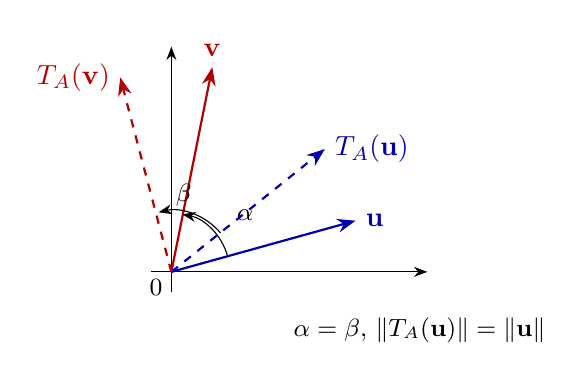
\begin{tikzpicture}[>=Stealth, scale=1.3]
  \draw[->] (-0.2,0) -- (2.5,0) node[right] {};
  \draw[->] (0,-0.2) -- (0,2.2) node[above] {};
  \node at (-0.15,-0.15) {\small $0$};
  \draw[->,thick,blue!70!black] (0,0) -- (1.8,0.5)
    node[right] {$\mathbf{u}$};
  \draw[->,thick,red!70!black] (0,0) -- (0.4,2.0)
    node[above] {$\mathbf{v}$};
  \draw[->] (0.55,0.15) arc[start angle=15,end angle=79,radius=0.57];
  \node at (0.72,0.55) {\small $\alpha$};
  \draw[->,thick,blue!70!black,dashed] (0,0) -- (1.5,1.2)
    node[right] {$T_A(\mathbf{u})$};
  \draw[->,thick,red!70!black,dashed] (0,0) -- (-0.5,1.9)
    node[left] {$T_A(\mathbf{v})$};
  \draw[->] (0.48,0.38) arc[start angle=40,end angle=103,radius=0.61];
  \node at (0.12,0.75) {\small $\beta$};
  \node[below right] at (1.1,-0.35)
    {\small $\alpha=\beta$, $\|T_A(\mathbf{u})\|=\|\mathbf{u}\|$};
\end{tikzpicture}
\caption{Orthogonal operator $T_A$ preserves norms and angles: $\beta = \alpha$.}
\label{fig:711}
\end{figure}

\redheading{Change of Orthonormal Basis}

Orthonormal bases are convenient because the following theorem shows that familiar formulas
continue to hold for norms, distances, and inner products when coordinates are computed
relative to such a basis.

\begin{tcolorbox}[colback=red!4, colframe=red!60!black,
  title={\textbf{Theorem 7.1.4}}, boxrule=0.5mm, arc=3mm]
If $S$ is an orthonormal basis for an $n$-dimensional inner product space $V$, and
\[
  (\mathbf{u})_S = (u_1,u_2,\ldots,u_n), \quad (\mathbf{v})_S = (v_1,v_2,\ldots,v_n)
\]
then:
\begin{enumerate}
  \item[(a)] $\|\mathbf{u}\| = \sqrt{u_1^2+u_2^2+\cdots+u_n^2}$
  \item[(b)] $d(\mathbf{u},\mathbf{v}) = \sqrt{(u_1-v_1)^2+(u_2-v_2)^2+\cdots+(u_n-v_n)^2}$
  \item[(c)] $\langle\mathbf{u},\mathbf{v}\rangle = u_1v_1+u_2v_2+\cdots+u_nv_n$
\end{enumerate}
\end{tcolorbox}

\textit{Remark.} The three parts can be restated as
\[
  \|\mathbf{u}\| = \|(\mathbf{u})_S\|, \qquad
  d(\mathbf{u},\mathbf{v}) = d\!\bigl((\mathbf{u})_S,(\mathbf{v})_S\bigr), \qquad
  \langle\mathbf{u},\mathbf{v}\rangle = \langle(\mathbf{u})_S,(\mathbf{v})_S\rangle
\]
so norms, distances, and inner products in $V$ equal those of the coordinate vectors
in $\mathbb{R}^n$ relative to any orthonormal basis.

Transitions between orthonormal bases for inner product spaces are of special importance
in geometry and applications. The following theorem characterizes the transition matrix.

\begin{tcolorbox}[colback=red!4, colframe=red!60!black,
  title={\textbf{Theorem 7.1.5}}, boxrule=0.5mm, arc=3mm]
Let $V$ be a finite-dimensional inner product space. If $P$ is the transition matrix
from one orthonormal basis $B'$ to another orthonormal basis $B$ for $V$, then $P$ is
an orthogonal matrix.
\end{tcolorbox}

\textit{Proof.} Let $\|\cdot\|_V$ denote the norm on $V$ and $\|\cdot\|$ the Euclidean norm on $\mathbb{R}^n$. Since $B'$ is an orthonormal basis, Theorem 7.1.4(a) gives for any $\mathbf{u}\in V$:
\[
  \|\mathbf{u}\|_V = \|[\mathbf{u}]_{B'}\| \tag{6}
\]
Let $\mathbf{x}$ be any vector in $\mathbb{R}^n$ and $\mathbf{u}$ the vector in $V$ with $[\mathbf{u}]_{B'} = \mathbf{x}$, so $P\mathbf{x} = [\mathbf{u}]_B$. Applying (6) to both bases:
\[
  \|\mathbf{u}\|_V = \|[\mathbf{u}]_{B'}\| = \|P\mathbf{x}\| \qquad\text{and}\qquad
  \|\mathbf{u}\|_V = \|[\mathbf{u}]_B\| = \|\mathbf{x}\|
\]
Therefore $\|P\mathbf{x}\| = \|\mathbf{x}\|$ for every $\mathbf{x}\in\mathbb{R}^n$, so $P$ is orthogonal by Theorem 7.1.3. $\blacksquare$

\redheading{Rotation Equations}

\subsection*{EXAMPLE 4 | Rotation of Axes in 2-Space}

When a rectangular $xy$-coordinate system is rotated counterclockwise through an angle
$\theta$ about the origin to produce an $x'y'$-system, each point $Q$ acquires two
sets of coordinates. Introducing unit vectors $\mathbf{u}_1, \mathbf{u}_2$ along the
$x$-, $y$-axes and $\mathbf{u}_1', \mathbf{u}_2'$ along the $x'$-, $y'$-axes, this is a
basis change from $B=\{\mathbf{u}_1,\mathbf{u}_2\}$ to $B'=\{\mathbf{u}_1',\mathbf{u}_2'\}$.
Using Formulas (7)--(8) of Section 4.7 one deduces
\[
  [\mathbf{u}_1]_{B'} = \begin{bmatrix}\cos\theta\\-\sin\theta\end{bmatrix}, \qquad
  [\mathbf{u}_2]_{B'} = \begin{bmatrix}\sin\theta\\\cos\theta\end{bmatrix}
\]
so the transition matrix and the \textbf{rotation equations} are

\begin{equation}
  \begin{bmatrix}x'\\y'\end{bmatrix}
  = P\begin{bmatrix}x\\y\end{bmatrix}, \qquad
  P = \begin{bmatrix}\cos\theta & \sin\theta\\-\sin\theta & \cos\theta\end{bmatrix}
  \tag{4}
\end{equation}

\noindent or equivalently,
\[
  \boxed{x' = x\cos\theta + y\sin\theta, \qquad y' = -x\sin\theta + y\cos\theta}
  \tag{5}
\]

By Theorem 7.1.5, $P$ is orthogonal, as can be verified directly.

\begin{figure}[h]
\centering
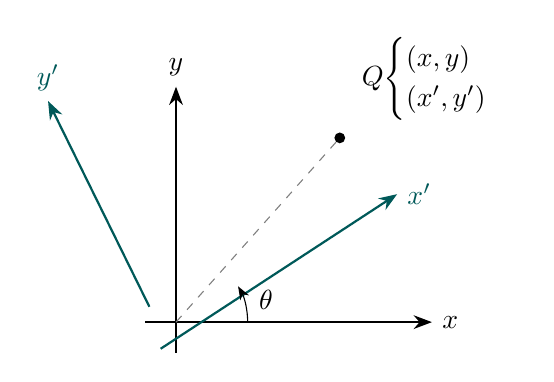
\begin{tikzpicture}[>=Stealth, scale=1.3]
  \draw[->,thick] (-0.3,0)--(2.5,0) node[right]{$x$};
  \draw[->,thick] (0,-0.3)--(0,2.3) node[above]{$y$};
  \draw[->,thick,teal!70!black] (-0.15,-0.26)--(2.16,1.25)
    node[right]{$x'$};
  \draw[->,thick,teal!70!black] (-0.26,0.15)--(-1.25,2.16)
    node[above]{$y'$};
  \draw[->] (0.7,0) arc[start angle=0, end angle=30, radius=0.7];
  \node at (0.88,0.22) {$\theta$};
  \fill (1.6,1.8) circle (1.5pt);
  \node at (1.72,1.88) [above right] {$Q\!\begin{cases}(x,y)\\(x',y')\end{cases}$};
  \draw[dashed,gray] (0,0)--(1.6,1.8);
\end{tikzpicture}
\caption{Rotation of the $xy$-axes through angle $\theta$ giving $x'y'$-coordinates.}
\end{figure}

\subsection*{EXAMPLE 5 | Rotation of Axes in 2-Space}

\textbf{SOLUTION:} Find the new coordinates of $Q(2,-1)$ after rotating the axes through
$\theta=\pi/4$. Since $\sin(\pi/4)=\cos(\pi/4)=1/\sqrt{2}$, equation (4) gives:
\[
  \begin{bmatrix}x'\\y'\end{bmatrix}
  = \begin{bmatrix}\tfrac{1}{\sqrt{2}} & \tfrac{1}{\sqrt{2}}\\[4pt]
                   -\tfrac{1}{\sqrt{2}} & \tfrac{1}{\sqrt{2}}\end{bmatrix}
    \begin{bmatrix}2\\-1\end{bmatrix}
  = \begin{bmatrix}\tfrac{1}{\sqrt{2}}\\[4pt]-\tfrac{3}{\sqrt{2}}\end{bmatrix}
\]
So the new coordinates of $Q$ are $\bigl(\tfrac{1}{\sqrt{2}},\,-\tfrac{3}{\sqrt{2}}\bigr)$.

\textit{Remark.} The coefficient matrix in (4) is the standard matrix for the linear
operator that rotates vectors through $-\theta$. Rotating the coordinate axes through
$\theta$ with vectors fixed has the same effect as rotating the vectors through $-\theta$
with the axes fixed.

\subsection*{EXAMPLE 6 | Rotation of Axes in 3-Space}

Suppose a rectangular $xyz$-system is rotated counterclockwise (looking down the positive
$z$-axis) through angle $\theta$ about the $z$-axis to produce an $x'y'z'$-system.
With unit vectors $\mathbf{u}_1,\mathbf{u}_2,\mathbf{u}_3$ along the $xyz$-axes and
$\mathbf{u}_1',\mathbf{u}_2',\mathbf{u}_3'$ along $x'y'z'$-axes:
\[
  [\mathbf{u}_1']_B = \begin{bmatrix}\cos\theta\\\sin\theta\\0\end{bmatrix}, \quad
  [\mathbf{u}_2']_B = \begin{bmatrix}-\sin\theta\\\cos\theta\\0\end{bmatrix}, \quad
  [\mathbf{u}_3']_B = \begin{bmatrix}0\\0\\1\end{bmatrix}
\]
The transition matrix from $B'$ to $B$ and its inverse are
\[
  P = \begin{bmatrix}\cos\theta & -\sin\theta & 0\\\sin\theta & \cos\theta & 0\\0 & 0 & 1\end{bmatrix},
  \qquad
  P^{-1} = \begin{bmatrix}\cos\theta & \sin\theta & 0\\-\sin\theta & \cos\theta & 0\\0 & 0 & 1\end{bmatrix}
\]
The new coordinates of a point $Q$ with old coordinates $(x,y,z)$ are:
\[
  \begin{bmatrix}x'\\y'\\z'\end{bmatrix}
  = \begin{bmatrix}\cos\theta & \sin\theta & 0\\-\sin\theta & \cos\theta & 0\\0 & 0 & 1\end{bmatrix}
    \begin{bmatrix}x\\y\\z\end{bmatrix}
\]

\begin{figure}[h]
\centering
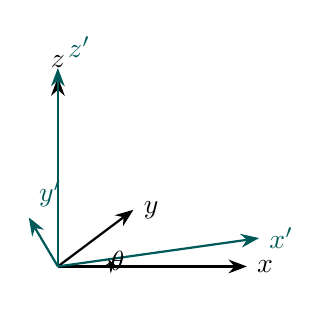
\begin{tikzpicture}[>=Stealth, scale=1.2]
  \begin{scope}[x={(1cm,0)},y={(0.4cm,0.3cm)},z={(0,1cm)}]
    \draw[->,thick] (0,0,0)--(2,0,0) node[right]{$x$};
    \draw[->,thick] (0,0,0)--(0,2,0) node[right]{$y$};
    \draw[->,thick] (0,0,0)--(0,0,2) node[above]{$z$};
    \draw[->,thick,teal!70!black] (0,0,0)--(1.73,1,0) node[right]{$x'$};
    \draw[->,thick,teal!70!black] (0,0,0)--(-1,1.73,0) node[above right]{$y'$};
    \draw[->,thick,teal!70!black] (0,0,0)--(0,0,2.1) node[above right]{$z'$};
    \draw[->] (0.5,0,0) arc[start angle=0,end angle=30,radius=0.5];
    \node at (0.55,0.2,0) {$\theta$};
  \end{scope}
\end{tikzpicture}
\caption{Rotation of the $xyz$-axes through angle $\theta$ about the $z$-axis.}
\end{figure}

\vspace{3mm}
\noindent\rule{\linewidth}{0.5pt}

\section*{Exercise Set 7.1}

\noindent\textit{In Exercises 1--4, determine whether the matrix is orthogonal, and if
so find its inverse.}

\begin{enumerate}

\item
\textbf{a.}\ $\begin{bmatrix}1&0\\0&-1\end{bmatrix}$
\hspace{20pt}
\textbf{b.}\ $\begin{bmatrix}\tfrac{1}{\sqrt{2}}&-\tfrac{1}{\sqrt{2}}\\[4pt]\tfrac{1}{\sqrt{2}}&\tfrac{1}{\sqrt{2}}\end{bmatrix}$

\item[3.]
\textbf{a.}\ $\begin{bmatrix}0&1&\tfrac{1}{\sqrt{2}}\\[4pt]1&0&0\\[4pt]0&0&\tfrac{1}{\sqrt{2}}\end{bmatrix}$
\hspace{15pt}
\textbf{b.}\ $\begin{bmatrix}-\tfrac{1}{\sqrt{2}}&\tfrac{1}{\sqrt{6}}&\tfrac{1}{\sqrt{3}}\\[4pt]0&-\tfrac{2}{\sqrt{6}}&\tfrac{1}{\sqrt{3}}\\[4pt]\tfrac{1}{\sqrt{2}}&\tfrac{1}{\sqrt{6}}&\tfrac{1}{\sqrt{3}}\end{bmatrix}$

\noindent\textit{In Exercises 5--6, show that the matrix is orthogonal three ways:
by computing $A^TA$, by using Theorem~7.1.1(b), and by using Theorem~7.1.1(c).}

\item[5.] $A = \begin{bmatrix}\tfrac{4}{5}&0&-\tfrac{3}{5}\\[4pt]-\tfrac{9}{25}&\tfrac{4}{5}&-\tfrac{12}{25}\\[4pt]\tfrac{12}{25}&\tfrac{3}{5}&\tfrac{16}{25}\end{bmatrix}$

\item[7.] Let $T_A\colon\mathbb{R}^3\to\mathbb{R}^3$ be multiplication by the orthogonal
matrix in Exercise~5. Find $T_A(\mathbf{x})$ for $\mathbf{x}=(-2,3,5)$, and confirm
that $\|T_A(\mathbf{x})\|=\|\mathbf{x}\|$ with the Euclidean inner product on $\mathbb{R}^3$.

\item[9.] Are the standard matrices for the reflections in Tables 1 and 2 of Section~1.8
orthogonal?

\item[11.] What conditions must $a$ and $b$ satisfy for the matrix
$\begin{bmatrix}a+b&b-a\\a-b&b+a\end{bmatrix}$
to be orthogonal?

\item[12.] Under what conditions will a diagonal matrix be orthogonal?

\noindent\textit{Exercises 13--14: find coordinates after rotation of axes.}

\item[13.] A rectangular $x'y'$-system is obtained by rotating the $xy$-system
counterclockwise through $\theta=\pi/3$.

\textbf{a.}\ Find the $x'y'$-coordinates of the point with $xy$-coordinates $(-2,6)$.

\textbf{b.}\ Find the $xy$-coordinates of the point with $x'y'$-coordinates $(5,2)$.

\item[15.] A rectangular $x'y'z'$-system is obtained by rotating the $xyz$-system
counterclockwise about the $z$-axis through $\theta=\pi/4$.

\textbf{a.}\ Find the $x'y'z'$-coordinates of the point with $xyz$-coordinates $(-1,2,5)$.

\textbf{b.}\ Find the $xyz$-coordinates of the point with $x'y'z'$-coordinates $(1,6,-3)$.

\item[21.] A linear operator on $\mathbb{R}^2$ is called \emph{rigid} if it does not
change lengths of vectors, and \emph{angle preserving} if it does not change the angle
between nonzero vectors.

\textbf{a.}\ Identify two different types of linear operators on $\mathbb{R}^2$ that are rigid.

\textbf{b.}\ Identify two different types that are angle preserving.

\textbf{c.}\ Are there any linear operators on $\mathbb{R}^2$ that are rigid but not angle
preserving? Justify your answer.

\item[24.] The sets $S=\{1,\,x\}$ and $S'=\bigl\{\tfrac{1}{\sqrt{2}}(1+x),\,\tfrac{1}{\sqrt{2}}(1-x)\bigr\}$
are orthonormal bases for $P_1$ with the standard inner product. Find the transition
matrix $P$ from $S$ to $S'$, and verify that the conclusion of Theorem~7.1.5 holds for $P$.

\item[25.] Prove that if $\mathbf{x}$ is an $n\times 1$ matrix, then
\[
  A = I_n - \frac{2}{\mathbf{x}^T\mathbf{x}}\,\mathbf{x}\mathbf{x}^T
\]
is both orthogonal and symmetric.

\item[26.] Prove that a $2\times 2$ orthogonal matrix $A$ has exactly two possible
forms:
\[
  A = \begin{bmatrix}\cos\theta & -\sin\theta\\\sin\theta & \cos\theta\end{bmatrix}
  \quad\text{or}\quad
  A = \begin{bmatrix}\cos\theta & \sin\theta\\\sin\theta & -\cos\theta\end{bmatrix}
\]
for some $0\le\theta<2\pi$. [\textit{Hint:} Start with a general $2\times 2$ matrix $A$
and use the fact that the column vectors form an orthonormal set in $\mathbb{R}^2$.]

\item[30.] Prove the equivalence of statements (a) and (c) in Theorem~7.1.1.

\end{enumerate}

\end{document}
